% SOICT 2026 submission — Springer CCIS format (single-blind: keep author names).
% Requires the Springer LNCS/CCIS class `llncs.cls` + `splncs04.bst` from
% https://soict.org/wp-content/uploads/2025/09/Latex-Template-for-Springer.zip
% Max 12 pages excluding references. Figure: docs/paper/diagrams/soict_harlstmgat.{pdf,png}.
%
% VERSION 2026-09-05 FINAL (simplified advisor report): VN100 primary + VN30 cross-market only;
%   HAR-X/LSTM/VolGA; delivered 22-fold/5-seed vol->Parkinson VolGA; all metrics; DM split per market
%   and contrast; contemp/estimator/pooled/HAR ablations removed.
% All numbers read from
%   results/walkforward_volga/walkforward_volga_{vn100,vn30}_h{1,5,10,22}.json (metrics[model].{mse,rmse,mae,qlike,r2}, dm_date_clustered)
% cross-checked against deliverables/2026-09-04_paper_pipeline_review/RESULTS_SUMMARY.md.
\documentclass[runningheads]{llncs}
\usepackage{graphicx}
\graphicspath{{diagrams/}}   % figure lives in docs/paper/diagrams/ (do NOT add ./ — collides with output pdf)
\usepackage{booktabs}
\usepackage{amsmath}
\usepackage{placeins}
\usepackage[T1]{fontenc}

\begin{document}

\title{VolGA: A Temporal Graph-Attention Model for Multi-Horizon Stock Volatility Forecasting in the Vietnamese Market}

\author{Author One\inst{1} \and Author Two\inst{1}}
\authorrunning{VolGA: Multi-Horizon Volatility Forecasting}
\institute{Affiliation, City, Country \\ \email{\{author1,author2\}@example.edu}}

\maketitle

\begin{abstract}
Forecasting daily stock-price volatility --- how much a stock's price is likely to swing on a given
day --- is a core input to risk management and option pricing: a risk manager sizing exposure or a
trader pricing an option needs to know not only where a price may go but how turbulent the path will
be.

We study \emph{VolGA} (Volatility Graph-Attention), a model that fuses a per-stock temporal branch
with a graph-attention branch, for multi-horizon volatility forecasting, using Vietnam's VN100 index
panel as the primary test market and the smaller VN30 panel as a cross-market study. All
feature-based models share the same five inputs and forecast a high--low range (Parkinson) measure of
daily variance at one, five, ten and twenty-two trading days ahead, against an extended HAR (HAR-X)
econometric benchmark and a same-feature no-graph LSTM that isolates the graph branch. Models are
compared with a leakage-free walk-forward protocol over twenty-two folds and five seeds on MSE, RMSE,
MAE, QLIKE and $R^2$, with a date-clustered Diebold--Mariano test that accounts for the
cross-sectional dependence of the panel. On VN100 at the daily horizon VolGA attains the lowest MSE,
RMSE and QLIKE and the highest $R^2$, and its absolute-error advantage over HAR-X is significant
($p<0.001$); relative to the no-graph LSTM the graph branch adds a significant QLIKE gain at the daily
and weekly horizons ($h1$: $p=0.008$; $h5$: $p=0.011$). At the longer horizons the linear HAR-X is the
strongest on QLIKE and MSE, where the models are otherwise close. On the smaller VN30 panel VolGA
leads on MSE, RMSE, MAE and $R^2$ at the daily horizon and its absolute-error advantage over HAR-X is
significant at the daily and weekly horizons ($p=0.002$, $p=0.009$), while HAR-X is the strongest on
QLIKE on the smaller panel. The graph branch contributes most on the broader, more liquid VN100 panel
at the short horizons.
\keywords{Volatility forecasting \and HAR \and LSTM \and Graph Attention Network \and Diebold--Mariano.}
\end{abstract}

\section{Introduction}
Financial markets are volatile: prices swing, and the size of those swings --- an asset's
\emph{volatility} --- is the standard measure of its risk. Because volatility drives how options
are priced, how much capital a position ties up, and how risk is budgeted across a portfolio,
forecasting it accurately is a long-standing problem in financial econometrics~\cite{corsi2009}.
Volatility is not observed directly; it is estimated from prices, so any forecast is a forecast of
an estimate. We target the daily \emph{Parkinson estimator}~\cite{parkinson1980}, which gauges a day's
variance from its high--low price range and uses more of the day's information than a close-to-close
measure; our
forecasting target is therefore a variance (a squared quantity), not a standard deviation.

The standard linear approach is the HAR family~\cite{corsi2009}: a plain linear regression that
predicts tomorrow's volatility from its own averages over the last day, the last week (about five
trading days), and the last month (about twenty-two), summarising volatility's long memory with a
handful of coefficients. This kind of model is deliberately simple yet provides a strong
low-complexity benchmark~\cite{corsi2009,audrino2025}; we adopt its extended form, HAR-X, which adds a
market factor and a volume regressor, as the linear benchmark throughout. HAR-X still treats each
stock on its own and ignores that stocks in the same market move together, so a shock in one stock is
never allowed to inform a forecast for another.

Two model families are widely proposed to close that gap. Sequence models such as the
LSTM~\cite{lstm1997} learn non-linear patterns in a stock's own history, and graph neural networks
--- here a Graph Attention Network (GAT)~\cite{gat2018} --- capture \emph{cross-sectional dependence},
the same-day co-movement of turbulence across related stocks, by letting each stock draw on an
attention-weighted average of its most relevant peers; the graph is a predictive device, not an
identified economic spillover mechanism. Whether these additions improve
out-of-sample volatility forecasts is mixed in the literature, and reported gains are often
confounded by evaluation choices --- for example counting many co-moving stocks as independent
evidence, which overstates statistical significance.

This paper asks \emph{where}, if anywhere, deep and graph models improve on the linear HAR-X
benchmark in the Vietnamese market. We take the VN100 index panel --- the larger, more liquid of the
two panels we study --- as the primary test market and the smaller VN30 panel as a cross-market
study, and, holding the five inputs and the data design fixed, compare the extended HAR-X, a no-graph
LSTM, and VolGA under one leakage-free walk-forward protocol so the only difference is the model. The
headline finding is stated plainly: on the VN100 panel VolGA is strongest at the daily horizon,
attaining the lowest MSE, RMSE and QLIKE and the highest $R^2$, and its directed
volume$\to$Parkinson graph adds a significant QLIKE gain over the same-feature no-graph LSTM at the
daily and weekly horizons ($h1$: $p=0.008$; $h5$: $p=0.011$); on the smaller VN30 panel VolGA again
leads on MSE, RMSE, MAE and $R^2$ at the daily horizon. Across both panels the linear HAR-X is the
strongest on QLIKE at the longer horizons, where the models are otherwise close, so the graph branch's
marginal value appears to track node breadth and liquidity.

Our contributions are: (i) a multi-horizon Vietnamese-market benchmark that holds the feature set
and data design fixed across HAR-X, a no-graph LSTM and VolGA on the VN100 and VN30 panels, so
any measured difference is attributable to a single component; (ii) the finding that VolGA delivers
the best daily-horizon accuracy across error metrics on both panels and that the graph branch's
contribution over the same-feature LSTM is significant on the larger, more liquid VN100 panel at the
short horizons; and (iii) a panel-correct significance
protocol --- because co-moving stocks are not independent, we cluster the Diebold--Mariano test by
date; ignoring this cross-sectional dependence can substantially overstate a test's
precision~\cite{petersen2009}. Every reported number is taken from a stored results file, and we document
the data-quality limitations --- notably the unverified split adjustment of the Vietnamese prices and
the variance (not standard-deviation) target --- rather than presenting the data as uniformly clean.

\paragraph{Terminology (for readers outside finance).}
\emph{Volatility}: the size of a stock's price fluctuations, the standard proxy for its risk.
\emph{Parkinson estimator}: a day's variance measured from its high--low price range; our
forecasting target is this variance (squared units), not the standard deviation.
\emph{HAR}: a linear model predicting volatility from its own daily, weekly, and monthly averages.
\emph{HAR-X}: HAR augmented with exogenous regressors~\cite{corsi2009,clements2024}.
\emph{GARCH}: a classical time-series model that carries variance forward from recent return shocks~\cite{bollerslev1986}.
\emph{QLIKE}: a proxy-robust error measure for volatility forecasts that stays reliable when the
target is a noisy proxy; in the ratio-based implementation used here its asymmetric shape makes
forecast under- and over-shoots matter differently~\cite{patton2011}.
\emph{Diebold--Mariano (DM) test}: a test of whether one forecast is more accurate than another by
more than chance, computed from their day-by-day loss differences.
\emph{Graph Attention Network (GAT)}: a model in which stocks are nodes and edges carry influence;
each stock updates from an attention-weighted average of its neighbours, capturing cross-stock
\emph{spillover}.
\emph{Horizon} $h$: how many trading days ahead we forecast ($h\in\{1,5,10,22\}$, roughly a day,
week, fortnight, and month).

\section{Related Work}
\textbf{HAR and classical models.} HAR~\cite{corsi2009} approximates the long memory of realized
volatility with a daily/weekly/monthly cascade; recent work reports that rolling-window and
specification choices, rather than model class, often account for measured differences from
HAR~\cite{audrino2025}. The ``-X'' extension augments HAR with exogenous regressors; the low-frequency
OHLC HAR-X of Clements, Preve and Tee~\cite{clements2024} validates a range-based target, and
network-augmented HAR-X analogues have been proposed~\cite{gnarharx2025}. HARQ~\cite{harq2016}
exploits measurement error, and GARCH-family models remain standard conditional-variance benchmarks;
we did not run GARCH in the present walk-forward and report it only as a reference class.
\textbf{Deep and graph models.} LSTMs~\cite{lstm1997} are widely applied to financial series, and
graph neural networks model cross-asset spillovers, e.g.\ Graph Attention Networks~\cite{gat2018},
multivariate realized-volatility GNNs~\cite{chen2022} and spillover-aware GNN-HAR
hybrids~\cite{gnnhar2025}; reported effects vary across studies and data designs. Volatility spillover
measurement has a long econometric tradition~\cite{dy2012}. \textbf{Graph construction.} Our graph
uses a directed volume$\to$Parkinson relation (each node attends to its Top-5 volume-shock leaders,
edge-weighted, over two hops), motivated by the documented volume--volatility
association~\cite{karpoff1987} and used here as a predictive design choice rather than a causal claim.
\textbf{Evaluation.}
Volatility is latent, so we use the proxy-robust QLIKE loss~\cite{patton2011} alongside MSE, with
significance by the Diebold--Mariano test~\cite{dm1995} and the Harvey--Leybourne--Newbold
small-sample correction~\cite{hln1997}.

\section{Method}
\textbf{Target and features.} The target is the Parkinson variance~\cite{parkinson1980} at day
$t{+}h$, a non-negative point forecast. The primary target is short-term, horizons $h\in\{1,5\}$
(one trading day and one trading week ahead); $h\in\{10,22\}$ (two weeks and roughly one trading
month) are an extended study. All three feature-based models (HAR-X, LSTM, VolGA) use the same five
node features per ticker at $t$: the daily Parkinson variance, its 5-day rolling mean (weekly), its
22-day rolling mean (monthly), a market Parkinson factor (the causal cross-sectional median of the
square-root Parkinson variance) and a 22-day volume z-score.

\textbf{Volatility estimator.} The target is the Parkinson variance. From the daily high $H$ and low
$L$ ($\ln$ is the natural logarithm), it estimates a day's variance from the high--low range:
\[
\sigma^2_{\mathrm{Park}} = \tfrac{1}{4\ln 2}\,\ln(H/L)^2 .
\]

\textbf{Models.} \emph{HAR-X} (linear benchmark~\cite{corsi2009,clements2024}): pooled OLS on the five
features (the daily/weekly/monthly cascade augmented with a market Parkinson factor and a volume
z-score), linear; its disclosed deviations from the canonical HAR-X are a range-based Parkinson target
and a direct single-day $t{+}h$ target. \emph{LSTM}: a two-layer LSTM (hidden 64) over the lookback
window of the five features; a single pooled model is trained over all tickers, each standardized by
its own scaler fit on training rows only, with a linear output inverse-transformed for evaluation
(dropout, weight decay, gradient clipping, ReduceLROnPlateau, early stopping). \emph{VolGA}
(Fig.~\ref{fig:arch}): the LSTM branch plus a Graph Attention Network branch~\cite{gat2018} that reads
the five node features at $t$ and attends over a directed volume$\to$Parkinson Top-5, edge-weighted,
two-hop graph estimated on training rows only; the branches are concatenated into an MLP head.
Comparing VolGA against the same-feature no-graph LSTM isolates the graph's contribution.

\textbf{Masked panel.} Not every stock is listed on every date. Rather than keep only the dates on
which all stocks trade (which discards most of the data), we keep every trading date and mask out
stocks not yet listed, with a mask-aware loss that ignores the masked stocks, so every model is
trained and evaluated on the same panel.

\textbf{Protocol.} We use an expanding-window walk-forward evaluation of twenty-two folds with a fixed
retrain cadence (a new model is fit every $K$ folds; the configuration is recorded in every results
file so the runs are reproducible), a lookback window of twenty-two trading days, and five seeds
(batch size $32$; the seed set is fixed across models). For the learned models we report, for each
metric, the seed-level metric summarised as the ensemble point value with the \emph{per-seed standard
deviation} on QLIKE, so seed sensitivity is visible rather than hidden by a seed-averaged prediction.
We report MSE, RMSE, MAE, QLIKE and $R^2$ with equal weight; predictions are floored at $10^{-2}$
times the
per-node training mean, applied identically to every model. Significance uses the
\emph{date-clustered} Diebold--Mariano test on the five-seed ensemble (mean) forecast: the
per-observation loss differential is collapsed to one value per calendar date before the statistic
(HLN correction, HAC lag $h{-}1$) is computed. This is the panel-correct treatment for a cross-section
that shares each trading date; a naive per-observation test treats the effective sample as the number
of tickers times the number of dates, which can substantially overstate precision when cross-sectional
dependence is ignored~\cite{petersen2009} --- under an independence approximation the overstatement
scales with about the square root of the number of stocks (of order ten on VN100, six on VN30), though
the exact factor depends on the panel's dependence structure. We report the targeted contrasts --- VolGA vs the
no-graph LSTM (the graph's marginal value) and VolGA vs HAR-X --- on QLIKE, squared error and
absolute error, because the verdict can be loss-dependent. Per-metric contrasts are reported without a
multiple-comparison correction (unadjusted).

\begin{figure}[t]
\centering
% figure generated by docs/paper/diagrams/generate_arch.py -> diagrams/soict_harlstmgat.{pdf,png,svg}
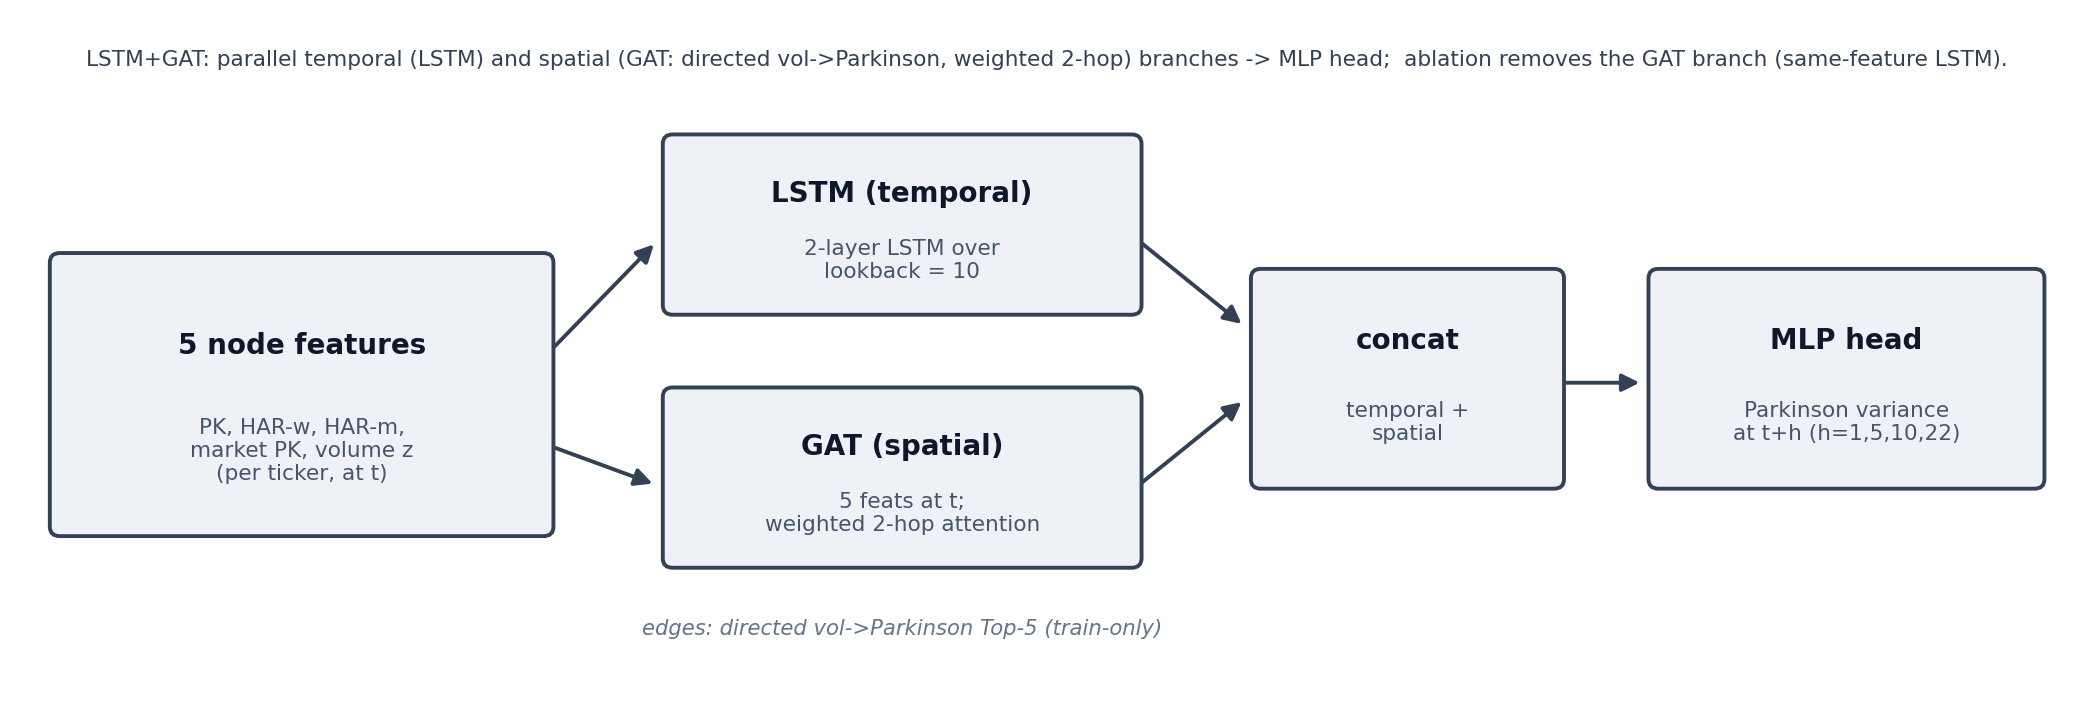
\includegraphics[width=\textwidth]{diagrams/soict_harlstmgat.png}
\caption{VolGA: a per-node LSTM temporal branch and a GAT spatial branch (directed volume$\to$Parkinson
Top-5 weighted two-hop attention) are concatenated into an MLP head; removing the GAT branch gives the
same-feature no-graph LSTM.}
\label{fig:arch}
\end{figure}

\section{Data}
The primary test market is the \textbf{VN100} index panel of the Vietnamese market (102 screened
tickers), the broader of the two panels; the \textbf{VN30} index panel (31 screened
tickers) serves as a cross-market study. Index membership follows the Ho Chi Minh Stock Exchange
index rules; both panels are additionally screened by trading history and liquidity, so ``broader''
refers to the larger, more actively traded VN100 constituent set. Both use the masked panel of Sec.~3
with the five features, per-ticker standardization fit on training rows only, and the walk-forward
protocol above. The VN100 test sample is
46{,}308 masked observations over 454 out-of-sample dates at $h1$; the VN30 test sample is 10{,}881
masked observations over 351 out-of-sample dates at $h1$.

\section{Experiments}
The main comparison is the extended linear benchmark HAR-X and the proposed model VolGA (directed
volume$\to$Parkinson weighted two-hop) on the primary VN100 panel at horizons $\{1,5,10,22\}$,
reporting MSE, RMSE, MAE, QLIKE and $R^2$ and the date-clustered Diebold--Mariano test
(Table~\ref{tab:vn100main}). The ablation then adds the no-graph LSTM to isolate the graph branch on
VN100 (Sec.~\ref{sec:graph}) and repeats the comparison on the smaller VN30 panel (Sec.~\ref{sec:vn30}).

\begin{table}[t]
\centering
\caption{Main result --- primary market VN100 panel ($N=102$; 46{,}308 masked obs over 454 test dates
at $h1$; 22 walk-forward folds, 5 seeds; VolGA: ensemble point value, QLIKE $\pm$~per-seed std). Lower
is better on every metric except $R^2$ (higher is better). MSE $\times10^{-7}$, RMSE/MAE
$\times10^{-4}$; QLIKE and $R^2$ unscaled.}
\label{tab:vn100main}
\footnotesize
\setlength{\tabcolsep}{6pt}
\begin{tabular}{llccccc}
\toprule
$h$ & Model & MSE & RMSE & MAE & QLIKE & $R^2$ \\
\midrule
1 & HAR-X & 2.363 & 4.861 & 2.850 & 0.5004 & 0.2248 \\
1 & VolGA & \textbf{2.348} & \textbf{4.846} & \textbf{2.816} & \textbf{0.4916}\,$\pm$\,0.0043 & \textbf{0.2297} \\
\midrule
5 & HAR-X & \textbf{2.602} & \textbf{5.101} & 3.113 & \textbf{0.5610} & \textbf{0.1477} \\
5 & VolGA & 2.615 & 5.114 & \textbf{3.067} & 0.5705\,$\pm$\,0.0144 & 0.1436 \\
\midrule
10 & HAR-X & \textbf{2.748} & \textbf{5.242} & 3.247 & \textbf{0.6001} & \textbf{0.1001} \\
10 & VolGA & 2.774 & 5.267 & \textbf{3.192} & 0.6149\,$\pm$\,0.0363 & 0.0916 \\
\midrule
22 & HAR-X & \textbf{2.883} & \textbf{5.370} & 3.428 & \textbf{0.6388} & \textbf{0.0570} \\
22 & VolGA & 2.913 & 5.397 & \textbf{3.352} & 0.6434\,$\pm$\,0.0031 & 0.0473 \\
\bottomrule
\end{tabular}
\end{table}

\section{Results: the VN100 market}\label{sec:results}
On the primary VN100 panel (Table~\ref{tab:vn100main}) VolGA is strongest at the daily horizon: it
attains the lowest MSE, RMSE and QLIKE ($h1$ QLIKE $0.4916$ vs HAR-X $0.5004$) and the highest $R^2$
($0.2297$ vs $0.2248$), and it has the lower MAE at every horizon. The date-clustered contrast against
HAR-X (Table~\ref{tab:dm-vn100-harx}) shows VolGA's absolute-error advantage is significant at the
short horizons ($h1$: $p<0.001$; $h5$: $p=0.005$; $h10$: $p=0.032$). At the weekly, fortnightly and
monthly horizons the linear HAR-X is the strongest on QLIKE and MSE, where the two models are
otherwise close, and the QLIKE difference between them is not statistically distinguishable at any
horizon ($p=0.177$, $0.585$, $0.520$, $0.842$). VolGA therefore delivers the best daily-horizon
accuracy across error metrics and a significant point-error reduction at the short horizons, with
HAR-X competitive on QLIKE at the longer horizons.

\FloatBarrier
\section{Ablation studies}\label{sec:abl}
\subsection{Graph component (VN100)}\label{sec:graph}
Adding the no-graph LSTM to the primary comparison isolates the graph branch: removing the GAT branch
from VolGA gives the same-feature no-graph LSTM (Table~\ref{tab:vn100graph}), so the VolGA-vs-LSTM
contrast measures the graph's marginal value (Table~\ref{tab:dm-vn100-lstm}). On VN100 the graph adds
a significant QLIKE gain over the no-graph LSTM at the daily horizon ($h1$: $p=0.008$) and the weekly
horizon ($h5$: $p=0.011$), and a significant absolute-error gain at the monthly horizon
($h22$: $p=0.016$); at $h10$ the two are not statistically distinguishable. Because the per-seed QLIKE
standard deviation of the learned models is in several cells of the same order as the graph-vs-LSTM
difference, and the DM test is computed on the five-seed ensemble forecast, the significant graph
effect on VN100 is best read as an ensemble-level regularity at the short horizons.

\begin{table}[t]
\centering
\caption{Graph ablation --- VN100 panel: HAR-X, the no-graph LSTM, and the full VolGA (same scaling
and sample as Table~\ref{tab:vn100main}; learned models: ensemble point value, QLIKE $\pm$~per-seed
std). Lower is better on every metric except $R^2$ (higher is better). MSE $\times10^{-7}$, RMSE/MAE
$\times10^{-4}$; QLIKE and $R^2$ unscaled.}
\label{tab:vn100graph}
\footnotesize
\setlength{\tabcolsep}{6pt}
\begin{tabular}{llccccc}
\toprule
$h$ & Model & MSE & RMSE & MAE & QLIKE & $R^2$ \\
\midrule
1 & HAR-X & 2.363 & 4.861 & 2.850 & 0.5004 & 0.2248 \\
1 & LSTM  & 2.355 & 4.853 & 2.821 & 0.5025\,$\pm$\,0.0223 & 0.2275 \\
1 & VolGA & \textbf{2.348} & \textbf{4.846} & \textbf{2.816} & \textbf{0.4916}\,$\pm$\,0.0043 & \textbf{0.2297} \\
\midrule
5 & HAR-X & \textbf{2.602} & \textbf{5.101} & 3.113 & \textbf{0.5610} & \textbf{0.1477} \\
5 & LSTM  & 2.621 & 5.119 & 3.068 & 0.5763\,$\pm$\,0.0170 & 0.1416 \\
5 & VolGA & 2.615 & 5.114 & \textbf{3.067} & 0.5705\,$\pm$\,0.0144 & 0.1436 \\
\midrule
10 & HAR-X & \textbf{2.748} & \textbf{5.242} & 3.247 & \textbf{0.6001} & \textbf{0.1001} \\
10 & LSTM  & 2.767 & 5.261 & \textbf{3.185} & 0.6096\,$\pm$\,0.0317 & 0.0936 \\
10 & VolGA & 2.774 & 5.267 & 3.192 & 0.6149\,$\pm$\,0.0363 & 0.0916 \\
\midrule
22 & HAR-X & \textbf{2.883} & \textbf{5.370} & 3.428 & \textbf{0.6388} & \textbf{0.0570} \\
22 & LSTM  & 2.921 & 5.404 & 3.370 & 0.6479\,$\pm$\,0.0076 & 0.0448 \\
22 & VolGA & 2.913 & 5.397 & \textbf{3.352} & 0.6434\,$\pm$\,0.0031 & 0.0473 \\
\bottomrule
\end{tabular}
\end{table}

\begin{table}[t]
\centering
\caption{Date-clustered DM contrasts on VN100 --- VolGA vs HAR-X ($p$-value; favoured model in
parentheses; bold when $p<0.05$; unadjusted; HLN correction, HAC lag $h{-}1$; date-clustered).
Reported on QLIKE, squared error (SE) and absolute error (AE).}
\label{tab:dm-vn100-harx}
\footnotesize
\setlength{\tabcolsep}{8pt}
\begin{tabular}{lccc}
\toprule
$h$ & QLIKE & SE & AE \\
\midrule
1  & 0.177 (VolGA) & 0.274 (VolGA) & \textbf{$<$0.001 (VolGA)} \\
5  & 0.585 (HAR-X) & 0.431 (HAR-X) & \textbf{0.005 (VolGA)} \\
10 & 0.520 (HAR-X) & 0.203 (HAR-X) & \textbf{0.032 (VolGA)} \\
22 & 0.842 (HAR-X) & 0.369 (HAR-X) & 0.094 (VolGA) \\
\bottomrule
\end{tabular}
\end{table}

\begin{table}[t]
\centering
\caption{Date-clustered DM contrasts on VN100 --- VolGA vs the same-feature no-graph LSTM (the graph's
marginal value; $p$-value; favoured model in parentheses; bold when $p<0.05$; unadjusted; HLN
correction, HAC lag $h{-}1$; date-clustered). Reported on QLIKE, squared error (SE) and absolute
error (AE).}
\label{tab:dm-vn100-lstm}
\footnotesize
\setlength{\tabcolsep}{8pt}
\begin{tabular}{lccc}
\toprule
$h$ & QLIKE & SE & AE \\
\midrule
1  & \textbf{0.008 (VolGA)} & 0.232 (VolGA) & 0.274 (VolGA) \\
5  & \textbf{0.011 (VolGA)} & 0.064 (VolGA) & 0.661 (VolGA) \\
10 & 0.229 (LSTM)           & 0.310 (LSTM)  & 0.251 (LSTM) \\
22 & 0.107 (VolGA)          & 0.147 (VolGA) & \textbf{0.016 (VolGA)} \\
\bottomrule
\end{tabular}
\end{table}

\subsection{Other market: VN30}\label{sec:vn30}
Repeating the comparison on the smaller VN30 panel (Table~\ref{tab:vn30}) VolGA again leads at the
daily horizon: it has the lowest MSE, RMSE and MAE and the highest $R^2$ at $h1$, and its
absolute-error advantage over HAR-X is significant at the daily and weekly horizons ($p=0.002$,
$p=0.009$; Table~\ref{tab:dm-vn30-harx}). On QLIKE the linear HAR-X is the strongest on this smaller
panel, and the QLIKE difference to VolGA is not statistically distinguishable at any horizon
($p=0.157$, $0.397$, $0.717$, $0.788$). The graph's marginal value over the no-graph LSTM
(Table~\ref{tab:dm-vn30-lstm}) is significant on squared and absolute error at the daily horizon
($p=0.032$, $p=0.005$) and on absolute error at $h10$ ($p=0.010$), while the QLIKE contrast is not
statistically distinguishable at any horizon. The graph branch thus contributes most on the broader,
more liquid VN100 panel at the short horizons.

\begin{table}[t]
\centering
\caption{Cross-market study --- VN30 panel ($N=31$; 10{,}881 masked obs over 351 test dates at $h1$;
22 folds, 5 seeds; learned models: ensemble point value, QLIKE $\pm$~per-seed std). Lower is better on
every metric except $R^2$ (higher is better). MSE $\times10^{-7}$, RMSE/MAE $\times10^{-4}$; QLIKE and
$R^2$ unscaled.}
\label{tab:vn30}
\footnotesize
\setlength{\tabcolsep}{6pt}
\begin{tabular}{llccccc}
\toprule
$h$ & Model & MSE & RMSE & MAE & QLIKE & $R^2$ \\
\midrule
1 & HAR-X & 1.938 & 4.402 & 2.402 & \textbf{0.4967} & 0.2310 \\
1 & LSTM  & 1.905 & 4.365 & 2.378 & 0.5219\,$\pm$\,0.0181 & 0.2439 \\
1 & VolGA & \textbf{1.890} & \textbf{4.348} & \textbf{2.362} & 0.5146\,$\pm$\,0.0071 & \textbf{0.2497} \\
\midrule
5 & HAR-X & 2.156 & 4.644 & 2.614 & \textbf{0.5937} & 0.1511 \\
5 & LSTM  & \textbf{2.130} & \textbf{4.616} & \textbf{2.564} & 0.6327\,$\pm$\,0.0247 & \textbf{0.1613} \\
5 & VolGA & 2.135 & 4.621 & 2.573 & 0.6150\,$\pm$\,0.0253 & 0.1595 \\
\midrule
10 & HAR-X & 2.363 & 4.861 & 2.771 & 0.6394 & 0.1083 \\
10 & LSTM  & \textbf{2.351} & \textbf{4.849} & 2.778 & \textbf{0.6336}\,$\pm$\,0.0048 & \textbf{0.1125} \\
10 & VolGA & 2.358 & 4.856 & \textbf{2.758} & 0.6485\,$\pm$\,0.1096 & 0.1101 \\
\midrule
22 & HAR-X & \textbf{2.751} & \textbf{5.245} & 3.015 & \textbf{0.6987} & \textbf{0.0699} \\
22 & LSTM  & 2.823 & 5.313 & \textbf{3.010} & 0.7056\,$\pm$\,0.0059 & 0.0456 \\
22 & VolGA & 2.829 & 5.319 & 3.011 & 0.7053\,$\pm$\,0.0042 & 0.0434 \\
\bottomrule
\end{tabular}
\end{table}

\begin{table}[t]
\centering
\caption{Date-clustered DM contrasts on VN30 --- VolGA vs HAR-X ($p$-value; favoured model in
parentheses; bold when $p<0.05$; unadjusted; HLN correction, HAC lag $h{-}1$; date-clustered).
Reported on QLIKE, squared error (SE) and absolute error (AE).}
\label{tab:dm-vn30-harx}
\footnotesize
\setlength{\tabcolsep}{8pt}
\begin{tabular}{lccc}
\toprule
$h$ & QLIKE & SE & AE \\
\midrule
1  & 0.157 (HAR-X) & 0.082 (VolGA) & \textbf{0.002 (VolGA)} \\
5  & 0.397 (HAR-X) & 0.154 (VolGA) & \textbf{0.009 (VolGA)} \\
10 & 0.717 (HAR-X) & 0.748 (VolGA) & 0.435 (VolGA) \\
22 & 0.788 (HAR-X) & 0.103 (HAR-X) & 0.874 (VolGA) \\
\bottomrule
\end{tabular}
\end{table}

\begin{table}[t]
\centering
\caption{Date-clustered DM contrasts on VN30 --- VolGA vs the same-feature no-graph LSTM (the graph's
marginal value; $p$-value; favoured model in parentheses; bold when $p<0.05$; unadjusted; HLN
correction, HAC lag $h{-}1$; date-clustered). Reported on QLIKE, squared error (SE) and absolute
error (AE).}
\label{tab:dm-vn30-lstm}
\footnotesize
\setlength{\tabcolsep}{8pt}
\begin{tabular}{lccc}
\toprule
$h$ & QLIKE & SE & AE \\
\midrule
1  & 0.179 (VolGA) & \textbf{0.032 (VolGA)} & \textbf{0.005 (VolGA)} \\
5  & 0.112 (VolGA) & 0.338 (LSTM)           & 0.052 (LSTM) \\
10 & 0.265 (LSTM)  & 0.484 (LSTM)           & \textbf{0.010 (VolGA)} \\
22 & 0.928 (VolGA) & 0.484 (LSTM)           & 0.963 (LSTM) \\
\bottomrule
\end{tabular}
\end{table}

\FloatBarrier
\section{Discussion}\label{sec:disc}
\textbf{Graph contribution.} The directed volume$\to$Parkinson graph adds a significant QLIKE gain
over the same-feature no-graph LSTM on the larger, more liquid VN100 panel at the daily and weekly
horizons (Table~\ref{tab:dm-vn100-lstm}); on VN30 the QLIKE contrast is not statistically
distinguishable from the no-graph LSTM at any horizon, though the graph is favoured on squared and
absolute error at the daily horizon (Sec.~\ref{sec:vn30}). The graph's marginal value is largest on
the broader, more actively traded VN100 panel. Because the per-seed QLIKE dispersion of the learned
models is in several cells of the same order as the graph-vs-LSTM difference, and the DM test is
computed on the five-seed ensemble forecast, the significant VN100 graph effect is best read as an
ensemble-level regularity at the short horizons.

\textbf{Parsimony against HAR-X.} On both panels the linear HAR-X is the strongest on QLIKE at most
horizons, and the QLIKE difference to the learned models is not statistically distinguishable at any
horizon (Table~\ref{tab:dm-vn100-harx}, Table~\ref{tab:dm-vn30-harx}); where the deep models
measurably improve on HAR-X is the absolute error, on which VolGA is significantly lower at the short
horizons (VN100 $h1$, $h5$, $h10$; VN30 $h1$, $h5$), and at the daily horizon VolGA also attains the
lowest MSE, RMSE and QLIKE and the highest $R^2$. This is consistent with the strength of HAR-X on
actively traded large-cap panels, where a smooth weighted average of recent volatility leaves limited
incremental room on the QLIKE loss in this sample.

\textbf{Loss dependence and multiplicity.} The ranking is metric- and horizon-dependent, which is why
all five metrics are reported: the daily horizon favours VolGA on MSE, RMSE, QLIKE and $R^2$, the
absolute-error comparison favours VolGA at the short horizons on both panels, and the graph-vs-LSTM
QLIKE comparison favours VolGA on VN100 at $h1$ and $h5$, while HAR-X is the strongest on QLIKE at the
longer horizons. We report per-metric DM contrasts without a multiple-comparison correction; the
significant absolute-error and VN100 graph results are reported with their exact $p$-values as
exploratory findings. \textbf{Inference design.} The
date-clustered DM test matters for these conclusions: a naive per-observation test on this
cross-sectionally dependent panel can substantially overstate precision~\cite{petersen2009} --- of
order the square root of the number of stocks under an independence approximation --- so a difference
that is not significant per date can appear significant per observation.
\textbf{Capacity.} VolGA adds a graph branch and its parameters to the no-graph LSTM, so this contrast
measures the effect of adding the implemented graph branch, not of graph structure at matched capacity.

\section{Limitations}
\emph{Split adjustment.} The raw Vietnamese prices are not split- or dividend-adjusted, so
overnight-based estimators inherit corporate-action jumps; we mitigate this by targeting the intraday
high--low Parkinson estimator, which is invariant to a common multiplicative split factor applied to
the day's high and low. This does not remove all corporate-action effects --- dividends, adjustments
that alter intraday fields, and erroneous OHLC records can still matter --- so the root fix would be
adjusted prices.
\emph{Variance target.} The forecasting target is a variance ($\sigma^2$), not a standard deviation
($\sigma$); QLIKE is applied to the variance with a positivity floor taken from the canonical
configuration, and forecast-error magnitudes are on the variance scale. \emph{Floor sensitivity.} The
QLIKE positivity floor interacts with high-zero-range days; floor sensitivity is more pronounced on
illiquid markets and is a documented caveat for any extension to such panels. \emph{Small $N$.} VN30
has only 31 nodes, so deep and graph methods are data-limited there, which is one reason the graph's
QLIKE contribution is weaker on VN30 than on the 102-node VN100. \emph{Scope.} The evidence is a
Vietnamese-market case study on two index panels; we do not generalise beyond the panels reported.

\section{Conclusion}
On the VN100 and VN30 panels of the Vietnamese market we benchmarked the extended linear HAR-X against
a no-graph LSTM and the temporal--graph VolGA model under one leakage-free walk-forward protocol with
the same features and a date-clustered Diebold--Mariano test. On the larger, more liquid VN100 panel
VolGA is strongest at the daily horizon --- lowest MSE, RMSE and QLIKE and highest $R^2$ --- and its
directed volume$\to$Parkinson graph adds a significant QLIKE gain over the same-feature no-graph LSTM
at the daily and weekly horizons; on VN30 VolGA leads on MSE, RMSE, MAE and $R^2$ at the daily
horizon, with a significant absolute-error advantage over HAR-X at the daily and weekly horizons.
Across both panels the linear HAR-X is the strongest on QLIKE at the longer horizons, where the models
are otherwise close, and the deep models' clearest advantage is a significant reduction in absolute
error at the short horizons. The practical takeaway is that, on these Vietnamese index panels, the
graph branch earns its keep on the broader, more liquid panel at the short horizons, where VolGA
delivers the best daily-horizon accuracy across error metrics.

\begin{thebibliography}{99}
\bibitem{corsi2009} Corsi, F.: A simple approximate long-memory model of realized volatility. J. Financial Econometrics \textbf{7}(2), 174--196 (2009)
\bibitem{parkinson1980} Parkinson, M.: The extreme value method for estimating the variance of the rate of return. J. Business \textbf{53}(1), 61--65 (1980)
\bibitem{yangzhang2000} Yang, D., Zhang, Q.: Drift-independent volatility estimation based on high, low, open, and close prices. J. Business \textbf{73}(3), 477--491 (2000)
\bibitem{rogers1991} Rogers, L.C.G., Satchell, S.E.: Estimating variance from high, low and closing prices. Ann. Appl. Probab. \textbf{1}(4), 504--512 (1991)
\bibitem{lstm1997} Hochreiter, S., Schmidhuber, J.: Long short-term memory. Neural Computation \textbf{9}(8), 1735--1780 (1997)
\bibitem{gat2018} Veli\v{c}kovi\'c, P., et al.: Graph attention networks. In: ICLR (2018)
\bibitem{dm1995} Diebold, F.X., Mariano, R.S.: Comparing predictive accuracy. J. Business \& Economic Statistics \textbf{13}(3), 253--263 (1995)
\bibitem{hln1997} Harvey, D., Leybourne, S., Newbold, P.: Testing the equality of prediction mean squared errors. Int. J. Forecasting \textbf{13}(2), 281--291 (1997)
\bibitem{patton2011} Patton, A.J.: Volatility forecast comparison using imperfect volatility proxies. J. Econometrics \textbf{160}(1), 246--256 (2011)
\bibitem{harq2016} Bollerslev, T., Patton, A.J., Quaedvlieg, R.: Exploiting the errors: a simple approach for improved volatility forecasting. J. Econometrics \textbf{192}(1), 1--18 (2016)
\bibitem{chen2022} Chen, Q., Robert, C.-Y.: Multivariate realized volatility forecasting with graph neural network. In: ACM ICAIF (2022). arXiv:2112.09015
\bibitem{gnnhar2025} Zhang, C., Pu, X., Cucuringu, M., Dong, X.: Forecasting realized volatility with spillover effects: perspectives from graph neural networks (2025). arXiv:2308.01419
\bibitem{dy2012} Diebold, F.X., Yilmaz, K.: Better to give than to receive: predictive directional measurement of volatility spillovers. Int. J. Forecasting \textbf{28}(1), 57--66 (2012)
\bibitem{audrino2025} Audrino, F., Chassot, J.: HARd to beat: the overlooked impact of rolling windows in the era of machine learning. Int. J. Forecasting (2025). arXiv:2406.08041
\bibitem{clements2024} Clements, A., Preve, D.P.A., Tee, C.: Harvesting the HAR-X volatility model. Working paper, SSRN 4733597 (2024)
\bibitem{gnarharx2025} \'O Nuall\'ain, T.: GNAR-HARX models for realised volatility: incorporating exogenous predictors and network effects (2025). arXiv:2510.24443
\bibitem{karpoff1987} Karpoff, J.M.: The relation between price changes and trading volume: a survey. J. Financial and Quantitative Analysis \textbf{22}(1), 109--126 (1987)
\bibitem{petersen2009} Petersen, M.A.: Estimating standard errors in finance panel data sets: comparing approaches. Review of Financial Studies \textbf{22}(1), 435--480 (2009)
\bibitem{bollerslev1986} Bollerslev, T.: Generalized autoregressive conditional heteroskedasticity. J. Econometrics \textbf{31}(3), 307--327 (1986)
\end{thebibliography}

\end{document}
